%!TEX root = ../thesis.tex
%*******************************************************************************
%*********************************** First Chapter *****************************
%*******************************************************************************

\chapter{Introduction}  %Title of the First Chapter

\ifpdf
    \graphicspath{{Chapter1/Figs/Raster/}{Chapter1/Figs/PDF/}{Chapter1/Figs/}}
\else
    \graphicspath{{Chapter1/Figs/Vector/}{Chapter1/Figs/}}
\fi

The completion of the Human Genome Project (HGP) \cite{Lander2001-du} and the advent of next-generation sequencing platform \cite{Bentley2008-kl} have made it possible to detect and analyse somatic mutations in thousands of tumours \cite{Weinstein2013-ko, ICGCTCGA_Pan-Cancer_Analysis_of_Whole_Genomes_Consortium2020-ts}. In contrast, the high cost associated with constructing high-quality reference genomes and the inability to detect somatic mutations in normal tissues at scale have hindered the characterisation of germline and somatic mutational processes across the tree of life, respectively. The ability to produce long and accurate reads through circular consensus sequencing (CCS) from Pacific Biosciences (PacBio) \cite{Wenger2019-pw} has sparked interest for \textit{de novo} assembly of genomes across the tree of life \cite{Darwin_Tree_of_Life_Project_Consortium2022-ma}. 

Here, I describe a new method that uses CCS reads to enable the detection of somatic mutations present as a single copy from bulk normal tissue. I discuss the application of this method to discovering new somatic mutational processes across in non-human samples.  Specifically, I leverage datasets and reference genomes generated through the Darwin Tree of Life (DToL) project to detect and analyse germline and somatic mutations, discover new mutational signatures, and investigate the conversation of these mutational signatures across the tree of life. Germline mutations are changes in the DNA that occur in the reproductive cells and are inherited by all cells of a progeny. In contrast, somatic mutations are changes in the DNA that occur in non-reproductive cells during an individual’s lifetime and are not inherited.

\section{The somatic mutation landscape of \textit{H. sapiens}}

The contribution of somatic mutations to oncogenesis was first implicated as early as 1890 by Friedrich von Hansemann, who observed aberrant chromosomal alterations in cancer cells under the microscope \cite{hansemann_1890}. Although most somatic mutations are benign (passenger mutations), some somatic mutations can confer a proliferative advantage to a cell (driver mutations). The detection of these driver mutations and their subsequent association with the hallmarks of cancer \cite{Hanahan2000-dp, Hanahan2011-zr} has been one of the primary motivations for cataloguing somatic mutations in tumours. The continued decline in sequencing costs and the concurrent development of somatic mutation detection algorithms have enabled the characterisation of somatic mutations in thousands of tumour samples \cite{Weinstein2013-ko, ICGCTCGA_Pan-Cancer_Analysis_of_Whole_Genomes_Consortium2020-ts}. In more past few years, somatic mutation detection in normal cells has become increasingly important to lineage trace embryonic development \cite{Behjati2014-gb} and to understand the transformation of normal cells to neoplastic cells \cite{Martincorena2015-io}. 

\subsection{Somatic mutation detection in tumours}
\label{sec:somatic_mutation_detection_in_tumours}

Cancer is often described as a disease of the genome. The acquisition of driver mutations through a single catastrophic event such as chromothripsis \cite{Stephens2011-gj} or gradual accumulation of somatic mutations \cite{Doll1954-of, Knudson1971-fg} is one of the primary contributors to tumourigenesis. Hence, somatic mutation detection is often the first step towards characterising the cancer genome. 

Unlike germline mutations, where approximately 50\% and 100\% of reads support the germline mutation, somatic mutations in tumour tissues can have a variant allele fraction (VAF) that ranges from 0-100\% depending on sample purity, cell clonality and copy number changes. Given that tumour samples frequently consist of a mixture of normal and cancer cells, accurately measuring the variant allele fraction (VAF) of somatic mutations can pose a challenge. Additionally, the copy number of the chromosome can fluctuate substantially in the cancer genome as a result of chromothripsis \cite{Stephens2011-gj}, aberrant chromosomal alternations \cite{Albertson2003-lr, Frohling2008-uc} or loss of heterozygosity (LOH) \cite{Lasko1991-wq}. Moreover, library errors that damage the template molecule before sequencing, as well as genomic DNA (gDNA) contamination, are other critical factors that must be considered in somatic mutation detection.

Matched tumour-normal sequencing is often performed to distinguish germline mutations from somatic mutations and to detect somatic mutations present in a clone of cells. A matched normal also enables the calculation of tumour purity, the proportion of cancer cells in a tumour sample, which is another critical component that determines somatic mutation detection sensitivity. Germline mutations detected in the matched normal serves as a reference panel to determine whether the mutation detected in the tumour sample is a germline mutation or a somatic mutation. In cases where a tumour sample has low sequence coverage or low tumour purity, there is also a possibility of misclassifying heterozygous germline mutations as somatic mutations \cite{Cibulskis2013-gw}.

Each somatic mutation detection algorithm uses a unique strategy to calculate the normal contamination in tumour \cite{Cibulskis2011-tp}, tumour contamination in normal \cite{Taylor-Weiner2018-af} and to differentiate between somatic and germline mutations. For instance, VarScan2 uses a hard filter \cite{Koboldt2012-wd}, MuTect uses a likelihood ratio \cite{Cibulskis2013-gw}, and Strelka2 uses a mixture model \cite{Kim2018-qi} based on the number of reads supporting the somatic mutation candidate in the normal and tumour sample for somatic mutation classification. Since each somatic mutation detection algorithm exhibits varying sensitivity and specificity, as well as different strengths and weaknesses, a consensus somatic mutation call from different somatic mutation algorithms is often used for downstream sequence analysis \cite{Bailey2020-ou}.

During library preparation, DNA damage is introduced to the template molecule, and a cocktail of DNA damage repair enzymes is used to repair it. If DNA damage remains unrepaired or is incorrectly repaired, the template DNA molecule is permanently altered before sequencing. During the sequencing process, base quality (BQ) scores are assigned to individual bases to reflect the uncertainty of each base call. Somatic mutation detection algorithms rely on sequence coverage and BQ scores to calculate the genotype quality (GQ) score of a germline mutation \cite{McKenna2010-br, Li2011-ag} and the confidence with which the somatic mutation is called \cite{Cibulskis2013-gw}. 

Since sequencing instruments cannot determine whether a base in the template molecule is derived from  a library error or a somatic mutation, the BQ score does not necessarily indicate the probability that a non-reference base in a read is the result of a mutation. Consequently, low-frequency library errors are often misclassified as somatic mutations, requiring specialised filters to minimise the number of false positive mutations \cite{Costello2013-cz, Chen2017-ba}.

PCR amplification, DNA oxidation and DNA crosslinking (in formalin-fixed tissues) are commonly recognised sources of library errors \cite{Chen2017-ba}. The identification of oxidative DNA damage during sonication-based DNA fragmentation, and the characterisation of read features that facilitate the differentiation between artefactual mutations and somatic mutations, serves as an illustrative example \cite{Costello2013-cz}. Acoustic shearing of DNA oxidises guanine to 8-oxoguanine (8-oxoG), and the preferential pairing of 8-oxoG with adenine \cite{Shibutani1991-tw} is responsible for the generation of CCG>CAG/CGG>CTG transversions during PCR amplification \cite{Costello2013-cz}. The addition of DNA glycosylases during library preparation can mitigate the effect of DNA oxidation. Furthermore, the sequence context and orientation bias of the mutation can also be assessed to determine the extent of oxidative DNA damage in the library \cite{Costello2013-cz}.

The repeat content of the reference genome is another important factor for somatic mutation detection. Repetitive sequences account for approximately 50\% of the human genome \cite{Lander2001-du}. When the repeat length exceeds the read length, read aligners are unable to determine the precise location of the read within the reference genome, as it could have originated from any of the copies of the repetitive sequence in the genome \cite{Li2008-dt}. Therefore, accurate read placement requires repetitive sequences to be flanked with unique sequences that are not present elsewhere in the reference genome. Alignment errors in low sequence complexity regions are another common source of false positive mutations \cite{Li2014-ra}. As a result, both germline and somatic mutation detection algorithms discard mutations when the total number of mismatches adjacent to the called mutation candidate, within a defined window, exceeds a predefined threshold \cite{Cibulskis2013-gw, DePristo2011-vf}. Consequently, the reference genome is divided into callable and non-callable regions based on read mappability, and variant calling is often restricted to the callable regions of the genome \cite{1000_Genomes_Project_Consortium2012-rj}. Hence, clinically relevant genes located in non-callable regions are often excluded from analysis \cite{Wagner2022-ph}.

The completeness of the reference genome is another crucial factor to consider in somatic mutation detection. Even the human reference genome remains incomplete, with missing sequences, unplaced and unlocalized scaffolds, and misassemblies such as erroneous sequence collapse and expansion \cite{Schneider2017-yo}. Recently, the latest advances in sequencing and physical mapping technologies have enabled the construction of the telomere-to-telomere CHM13 (T2T-CHM13) genome, which represents the most accurate and complete human genome to date.  In comparison to the human reference genome, the T2T-CHM13 genome provides fully resolved sequences for the short arms of acrocentric chromosomes and the centromeres of all chromosomes, except for chromosome Y \cite{Nurk2022-dv}. As expected, the T2T-CHM13 genome significantly improves the accuracy and precision of both read alignment and variant calling \cite{Aganezov2022-dv}.

To account for errors that cannot be eliminated through an analytical approach, a panel of normal (PoN) VCF file is generated from a set of normal samples using the same parameters as those applied in somatic mutation detection. Afterwards, somatic mutation detections found in the PoN VCF are filtered out \cite{Cibulskis2013-gw}.

\subsection{Somatic mutation detection in normal tissue}
\label{sec:somatic_mutation_detection_in_normal_tissue}

In tumor samples, clonal somatic mutations with a variant allele fraction (VAF) above 0.1-1\%, exceeding the Illumina sequencing error rate \cite{Cibulskis2013-gw}, are detectable. Somatic mutations with a VAF below this threshold cannot be distinguished from background noise.

In contrast, somatic mutations in normal samples are typically present in only a few copies within DNA extracted from bulk normal tissue, presenting unique challenges for detection. To enable somatic mutation detection in normal tissues, the copy number of mutant DNA is increased above the detection threshold \cite{Lee-Six2018-qe}, or base accuracy is enhanced through upstream modifications to the library preparation protocol \cite{Schmitt2012-yr, Hoang2016-jx, Abascal2021-pk}.

\subsubsection{Single-cell resolution somatic mutation detection}

Both single-cell whole-genome amplification \cite{Lodato2018-hh} and single-cell clone expansion and sequencing \cite{Lee-Six2018-qe, MSpencer_Chapman2021-cq} aims to increase the copy number of the mutant DNA prior to library preparation and sequencing. On the other hand, laser-capture microdissection (LCM) and sequencing leverage spatial partitioning of tissues through histological staining to isolate and sequence a clonal unit of cells, such as the colonic crypt \cite{Ellis2021-it}. Single-cell clone expansion and LCM sequencing are recognised as the gold-standard methods for somatic mutation detection in single cells or clonal tissues, respectively. In contrast, single-cell whole-genome amplification and sequencing has several disadvantages. For instance, allele dropout occurs during PCR amplification when one of the two alleles at a heterozygous locus is not amplified, leading to a false homozygous mutation call. To date, single-cell clone expansion and LCM sequencing have been successfully used to determine the somatic mutation rate, the somatic mutational processes, and the clonal structure across a range across a range of normal tissues, including adrenal gland, blood, bladder, bronchus, cardiac muscle, colon, endometrium, oesophagus, pancreas, placenta, prostate, skin, smooth muscle, testis, thyroid, ureter, visceral fat \cite{Lee-Six2018-qe, MSpencer_Chapman2021-cq, Martincorena2015-gu, Ju2017-vw, Martincorena2018-av, Brunner2019-xg, Lee-Six2019-vt, Yoshida2020-yr, Olafsson2020-vi, Moore2020-pi, Lawson2020-em, Coorens2021-ct, Robinson2021-te, Grossmann2021-gd, Moore2021-dl, Park2021-fx, Ng2021-jd, Mitchell2022-ry}. 

\subsubsection{Single-molecule resolution somatic mutation detection}

At the heart of the double-stranded consensus sequencing method, is the unique molecular (UMI) barcode, 3 to 16 nucleotides attached to each DNA molecule, and the generation of multiple copies of the forward and reverse strand template molecule through PCR amplification. UMI barcode enables the differentiation of reads mapped to the same reference coordinate and the identification of reads derived from the same molecule. Redundancies between the copies of the same template molecule is used to generate a highly accurate consensus sequence, and complementary base pairing between the forward and reverse strand of a double-stranded molecule is used to correct library errors or PCR amplification errors that occur on one of the two strands \cite{Schmitt2012-yr, Hoang2016-jx, Abascal2021-pk}. Duplex reads generated from the above method has a reported error rate of 2 errors per 10 million bases \cite{Schmitt2012-yr}. Recently, a new duplex sequencing protocol called nanorate sequencing protocol was developed to address library errors occurring on both strands of a double-stranded DNA molecule, thereby reducing the duplex read error rate to 5 errors per 1 billion bases, and enabling single-molecule resolution somatic mutation detection \cite{Abascal2021-pk}.

\subsection{Somatic mutations as biological barcodes}

Somatic mutations accumulate throughout life. The acquisition of the first few somatic mutations begins with the first cell division of an embryo, and daughter cells inherit these mutations during embryogenesis \cite{Ju2017-vw}. Somatic mutations acquired during embryonic development are often referred to as mosaic mutations because cells with these mutations are distributed in a mosaic fashion across the adult body. The pattern of their distribution depends on the timing and stem cell lineage in which the mutation occurred. 

Similar to how UMI barcodes are used to distinguish unique molecules, mosaic mutations can also function as biological barcodes. Daughter cells that share the same somatic mutation can be assumed to have the same haplotype – a group of alleles on a single chromosome – and therefore are derived from the same stem cell lineage. To date, somatic mutations have been successfully used to trace the cellular origin of different tissues, and measure the approximate time at which various lineages separated, and gain deeper insights into the complexities of embryonic development \cite{Behjati2014-gb}.

For example, the gradual accumulation of somatic mutations is often proposed as a key factor in tumorigenesis in adult tumours. In contrast, paediatric tumours have had insufficient time to accumulate such mutations. As an alternative hypothesis, abnormal embryonic development has been proposed as an alternative explanation \cite{Marshall2014-ec}. If paediatric cancers are derived from gradual accumulation of somatic mutations, paediatric cancers will have a unique set of somatic mutations, independent of their tissue of origin. However, if paediatric cancers are the result of aberrant embryonic development, pediatric cancers and premalignant clones will share mosaic mutations with the neighbouring normal tissue. 

The study of shared somatic mutations in bilateral and unilateral Wilms tumour and adjacent normal kidney tissues supports the hypothesis that paediatric cancer arises from abnormal embryonic development \cite{Coorens2019-zf}. A similar analysis in bilateral adrenal neuroblastoma also revealed that the left and right adrenal gland tumours do not arise from a single premalignant clone. Instead two independent premalignant clones separated before the first few cell divisions of a zygote and developed into two independent tumours \cite{Coorens2020-ut}. Intriguingly, these two studies also show that the left-right axis of the kidneys and adrenal glands are established during the first few cell divisions of a zygote.

\subsection{Somatic mutational processes}
\label{sec:mutational_signature_analysis}

Somatic mutational process is a continuous process throughout life, and multiple somatic mutational processes simultaneously act on the cell’s genome at any given time. Mutational signature analysis is performed to determine the somatic mutational processes that have acted upon the genome and measure the contribution of each somatic mutational process to the mutational burden of the sample. Mutational signature analysis can either \textit{de novo} extract new mutational signatures from a catalogue of somatic mutations from multiple samples or use a set of reference mutational signatures to calculate the attribution of each mutational signature to the mutation burden of the sample. A mutational signature is defined as a set of probabilities that represent the likelihood of a somatic mutational process to generate a mutation at a specific sequence context \cite{Alexandrov2013-fq}.

During mutational signature analysis, somatic mutations are classified according to the event, the size of the event and the sequence context. For example, single base substitutions (SBS) are often classified using the SBS96 classification system. In the pyrimidine context, there are 6 types of substitutions (C>A, C>G, C>T, T>A, T>C and T>G) and 16 possible trinucleotide contexts derived from the 4 bases upstream and downstream of the substitution. This combination of substitutions and trinucleotide contexts defines the canonical SBS96 classification system. 

The SBS96 classification system can be further expanded to the SBS192 or the SBS1536 classification. The SBS192 classification system considers whether the somatic mutation has occurred on the transcribed or untranscribed strand of the gene to assess whether the somatic mutation is associated with transcription-coupled damage or repair. On the other hand, the SBS1536 classification system expands the trinucleotide context to a pentanucleotide context to evaluate each somatic mutation in greater detail. 

Additional somatic mutation classification systems exist for double base substitution (DBS), insertions and deletions (indels) and structural variations, but they are not the primary focus of this PhD thesis \cite{Alexandrov2013-kg, Alexandrov2020-ys, Li2020-vw, Steele2022-mn}.

The PCAWG consortium has discovered 67 SBS mutational signatures \cite{Alexandrov2020-ys} and the biological aetiology has been determined for 49 SBS mutational signatures (Table \ref{tab:pcawg-mutational-signatures}). 

\begingroup
\setlength{\LTleft}{-10cm plus -1fill} %% centering
\setlength{\LTright}{\LTleft}
\begin{longtable}{c|p{10cm}|c}
\label{tab:pcawg-mutational-signatures} \\ \smallskip
Mutational Signature & Aetiology & Reference \\ \hline

SBS1 & Spontaneous deamination of 5-methylcytosine to thymine & \cite{Alexandrov2015-db} \\ \hline
SBS2 & APOBEC mutagenesis & \cite{Burns2013-xn} \\ \hline
SBS3 & Defective homologous recombination-based DNA damage repair & \cite{Zamborszky2017-ma} \\ \hline
SBS4 & Tobacco smoking & \cite{Alexandrov2016-uw} \\ \hline
SBS5 & - & \cite{Alexandrov2015-db} \\ \hline
SBS6 & Defective DNA mismatch repair & \cite{Meier2018-cj} \\ \hline
SBS7abcd & UV light exposure & \cite{Nik-Zainal2015-bj} \\ \hline
SBS8 & - & \\ \hline
SBS9 & POLE mutagenesis & - \\ \hline
SBS10ab & POLE mutagenesis & \cite{Robinson2021-te} \\ \hline
SBS10cd & POLD mutagenesis & \cite{Robinson2021-te} \\ \hline
SBS11 & Temozolomide treatment & \cite{Kucab2019-fy} \\ \hline
SBS12 & - & - \\ \hline
SBS13 & APOBEC3A mutagenesis & \cite{Chan2015-sk} \\ \hline
SBS14 & POLE mutagenesis and defective DNA mismatch repair & \cite{Hodel2020-je} \\ \hline
SBS15 & Defective DNA mismatch repair & \cite{Meier2018-cj} \\ \hline
SBS16 & - & - \\ \hline
SBS17ab & - & - \\ \hline
SBS18 & Oxidative DNA damage & \cite{Kucab2019-fy} \\ \hline
SBS19 & - & - \\ \hline
SBS20 & POLD mutagenesis and defective DNA mismatch repair  & \cite{Meier2018-cj} \\ \hline
SBS21 & Defective DNA mismatch repair & \cite{Meier2018-cj} \\ \hline
SBS22 & Aristolochic acid exposure & \cite{Nik-Zainal2015-bj} \\ \hline
SBS23 & - & - \\ \hline
SBS24 & Aflatoxin exposure &  \cite{Chawanthayatham2017-oh} \\ \hline
SBS25 & Chemotherapy treatment & - \\ \hline
SBS26 & Defective DNA mismatch repair &  \cite{Meier2018-cj} \\ \hline
SBS28 & - & - \\ \hline
SBS29 & Tobacco chewing & - \\ \hline
SBS30 & Defective DNA base excision repair due to NTHL1 mutations &  \cite{Drost2017-xw} \\ \hline
SBS31 & Platinum chemotherapy treatment & \cite{Boot2018-gv} \\ \hline
SBS32 & Azathioprine treatment & \cite{Inman2018-fh} \\ \hline
SBS33 & - & - \\ \hline
SBS34 & - & - \\ \hline
SBS35 & Platinum chemotherapy treatment & \cite{Boot2018-gv} \\ \hline
SBS36 & Defective DNA base excision repair due to MUTYH mutations & \cite{Pilati2017-mx} \\ \hline
SBS37 & - &  - \\ \hline
SBS38 & Indirect effect of UV light & - \\ \hline
SBS39 & - & - \\ \hline
SBS40 & - & - \\ \hline
SBS41 & - & - \\ \hline
SBS42 & Haloalkane exposure &  \cite{Mimaki2016-kh} \\ \hline
SBS44 & Defective DNA mismatch repair & \cite{Drost2017-xw} \\ \hline
SBS84 & Activity of activation-induced cytidine deaminase (AID) & - \\ \hline
SBS85 & Indirect effects of activity of AID & - \\ \hline
SBS86 & Unknown chemotherapy treatment & - \\ \hline
SBS87 & Thiopurine chemotherapy treatment & \cite{Li2020-re} \\ \hline
SBS88 & Colibactin exposure &  \cite{Pleguezuelos-Manzano2020-er} \\ \hline
SBS89 & - & - \\ \hline
SBS90 & Duocarmycin exposure &  \cite{Boot2020-gg} \\ \hline
SBS91 & - & -\\ \hline
SBS92 & Tobacco smoking & - \\ \hline
SBS93 & - & - \\ \hline
SBS94 & - & - \\ \hline
\caption{COSMIC mutational signatures}
% \floatfoot{If a mutational process has been identified for the mutational signature through external experimental validation, citations have been provided. There are several mutational signatures where both the cause and aetiology of the mutation is unknown.}
\end{longtable}
\endgroup

The mutational signatures listed here are not an exhaustive list of all the discovered SBS mutational signatures. If a mutational process has been identified for the mutational signature through external experimental validation, citations have been provided. 

Ongoing research continues to find new somatic mutational signatures and determine the aetiology of these mutational signatures. For instance, Genomics England and collaborators have leveraged 100,000 cancer genomes from around 85,000 patients to detect mutational signatures associated with rare and sporadic somatic mutagenesis \cite{Degasperi2022-qe}. Somatic mutations resulting from chemotherapeutic agents is another active area of research \cite{Pich2019-ja, Aitken2020-sa}. 

\section{Single molecule sequencing}

Unlike the sequencing by synthesis from Illumina, single-molecule sequencing from Oxford Nanopore Technologies (ONT) and Pacific Biosciences (PacBio) determines the nucleotide composition of an individual DNA molecule. Here, I focus on the past, present and future of single-molecule real-time (SMRT) sequencing platform from PacBio. 

During the early years of development, SMRT sequencing promised the following potential benefits \cite{}:

\begin{enumerate}
\item lower input material for library preparation and sequencing
\item higher base accuracy
\item longer read length (10kb – 100kb)
\item production of contigs with higher N50
\item nucleotide-resolution identification of structural variations. 
\item simultaneous detection of genetic variations and base modifications
\end{enumerate}

The first generation of PacBio sequencing instruments failed to meet the above expectations. Concurrently, Illumina developed sequencing instruments that generated shorter reads with higher base accuracy, as well as a lower cost per base for sequencing \cite{Bentley2008-kl}. Consequently, sequencing by synthesis from Illumina quickly became the primary sequencing method. Lately, SMRT sequencing has started to fulfil some of the promises with improvements in both read length and base accuracy. In this section, I discuss the advances in the SMRT sequencing platform and expanding list of applications. 

\subsection{Single-molecule real-time sequencing}

PacBio was founded in 2004 with the aspiration of commercialising the SMRT sequencing technology developed at Cornell University. At the heart of the SMRT platform lies the zero-mode-waveguide (ZMW), a nano-scaled hole fabricated in a metal film. The ZMW functions as the sequencing unit and its unique properties helps the SMRT platform achieve the high signal-to-noise ratio necessary for observing the activity of individual DNA polymerases (DNAP) \cite{Levene2003-og}. 

The metal film with the ZMW is positioned on top of a glass, while the DNAP is immobilised at the bottom glass surface through surface chemistry modifications. These modifications prevent the adsorption of DNAP to the metal side walls \cite{Korlach2008-aq, Eid2009-ol}. A topologically circular template, also known as a SMRTbell template, is created through the attachment of hairpin adapters to a double-stranded DNA molecule (Figure \ref{figure:smrtbell-template}).

\begin{figure}[htbp!]
\caption{SMRTbell template}
\label{figure:smrtbell-template}
\begin{centering}
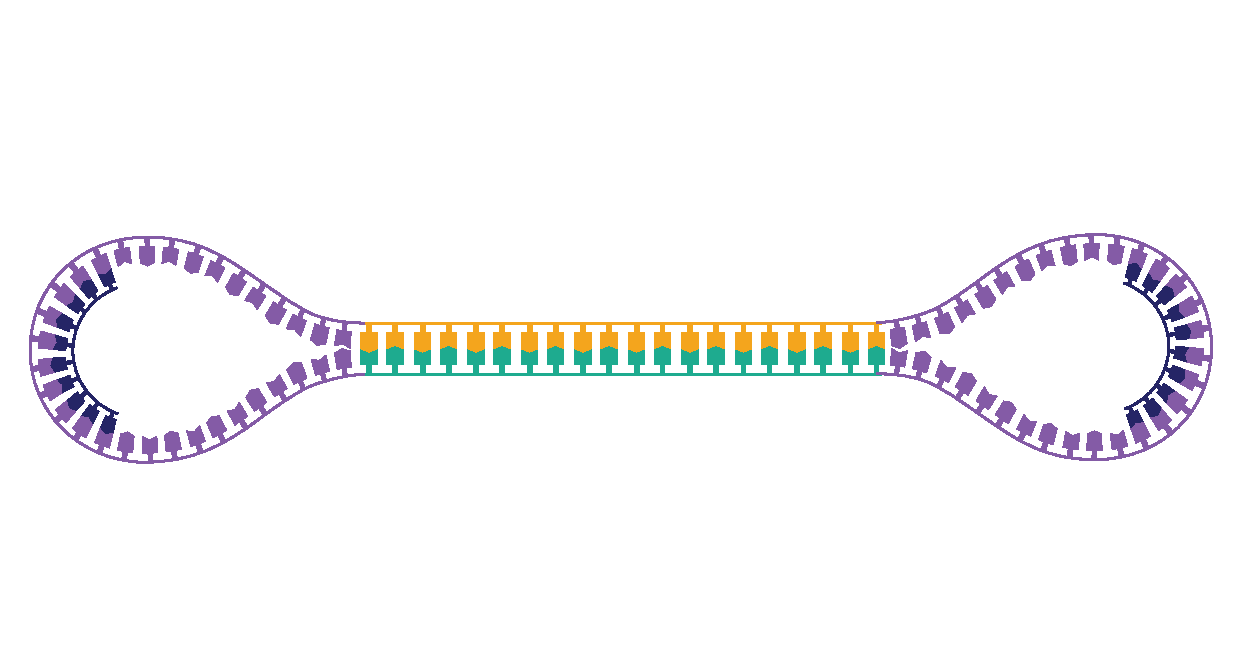
\includegraphics[width=\textwidth]{Vector/SMRTbell_template.pdf}
\end{centering}
\floatfoot{A hairpin adapter in purple is attached to a double-stranded DNA. The forward strand is coloured in yellow and reverse strand is coloured in green. The primer that DNAP binds to is coloured in black.}
\end{figure}

The loading of SMRTbell template into a ZMW follows a Poisson distribution, and typically 30-50\% of the ZMWs are classified as productive ZMWs, where a single DNAP successfully initiates and completes rolling circle sequencing. SMRT sequencing initially used $\Phi$29 DNAP due to its high processivity, minimal amplification bias and ability to perform strand displacement DNA synthesis \cite{Eid2009-ol}. Additionally, $\Phi$29 DNAP was engineered through site-directed mutagenesis to enable the incorporation of fluorophore-labelled deoxyribonucleoside triphosphate (dNTP) during DNA elongation \cite{Eid2009-ol, Korlach2008-fv}. 

After the successful loading of the SMRTbell template, free nucleotides are released above the ZMW array, and they diffuse in and out of the ZMW. DNAP binds to the template and incorporates the correct nucleotide into the growing DNA strand. Upon nucleotide incorporation, DNAP cleaves the fluorophore from the nucleotide, resulting in the synthesis of a native DNA molecule. DNAP continues DNA elongation until DNA replication is terminated.

The length of the DNA synthesis is dependent on DNAP processivity and the presence of bulky DNA damage on the template DNA, which can cause premature termination of DNA replication. Illumination from the laser below the glass surface excites the fluorophore, and the emitted fluorescence is measured. An image processor leverages the temporal difference between the diffusion of free nucleotides (which occurs in microseconds) and nucleotide incorporation (which occurs in milliseconds) to distinguish the background fluorescence from free nucleotides and fluorescence from nucleotide bound to DNAP. Critically, the size and shape of the ZMW prevents laser light from passing through the ZMW, confining the illumination to the bottom of the ZMW and improving the signal-to-noise ratio. As the four dNTPs are each labelled with a different fluorophore, each nucleotide can be identified from their unique fluorescence \cite{Eid2009-ol}. 

DNAP kinetics can also be used to detect DNA base modifications. DNAP kinetics is comprised of duration of fluorescence pulse, known as pulse width, and the duration between successive fluorescence pulses, referred to as interpulse duration (IPD) \cite{Flusberg2010-ub}. To date, DNAP kinetics has been used to detect base modifications such as N6-methyladenine, 5-methylcytosine (5mC) and 5-hydroxymethylcytosine \cite{Flusberg2010-ub} and DNA damage such as O6-mmethylguanine, 1-methyladenine, O4-methylthymien, 5-hydroxycyostine, 5hydroxyuracil, 5-hydroxymethyluyracil and thymine dimers \cite{Clark2011-jz}. 

The PacBio RS instrument, equipped with the first generation of polymerase and chemistry (P1-C1), and the first generation of SMRTcells with 150,000 ZMWs \cite{Rhoads2015-pk} produced CLR reads with an error rate of 10-15\% and an average length of 1,500 bp \cite{Eid2009-ol, Quail2012-cx}. The earlier PacBio sequencing instruments were unable to produce longer and more accurate reads because of insufficient DNAP processivity, which is a measure of the rate at which DNAP performs DNA synthesis, and a constraint on instrument running time of 20-30 hours. 

To increase base accuracy of long reads, PacBio developed the circular consensus sequencing (CCS) method in 2010, which leverages rolling circle sequencing to obtain multiple copies of the forward and reverse strand of the template molecule to generate a more accurate CCS read \cite{} (Figure \ref{figure:clr-sequencing}. Because there is an inherent trade-off between read length and base accuracy, while maintaining DNAP processivity as a constant, the earlier PacBio sequencing instruments were not able to produce CCS reads longer than 1-2kb (i.e., earlier generation of DNAP did not have the processivity to sequence both the forward and reverse strand of a SMRTbell template with a longer read-of-insert (>10kb) multiple times). Consequently, the generation of longer CLR reads was preferred to shorter, but more accurate CCS reads with the earlier PacBio sequencing instruments. Unfortunately, the high error rate of CLR sequencing greatly limited the scope of its applications. 

% To increase base accuracy of long reads, PacBio developed the circular consensus sequencing (CCS) method in 2010, which leverages rolling circle sequencing to obtain multiple copies of the forward and reverse strand of the template molecule to generate a more accurate CCS read \cite{} (Figure \ref{figure:clr-sequencing}. Because there is an inherent trade-off between read length and base accuracy, while maintaining DNAP processivity as a constant, the earlier PacBio sequencing instruments were not able to produce CCS reads longer than 1-2kb (i.e., earlier generation of DNAP did not have the processivity to sequence both the forward and reverse strand of a SMRTbell template with a longer read-of-insert (>10kb) multiple times). Consequently, the generation of longer CLR reads was preferred to shorter, but more accurate CCS reads with the earlier PacBio sequencing instruments. Unfortunately, the high error rate of CLR sequencing greatly limited the scope of its applications \ref{\section{}}.

\begin{figure}[h!]
\caption{CLR sequencing}
\label{figure:clr-sequencing}
\begin{centering}
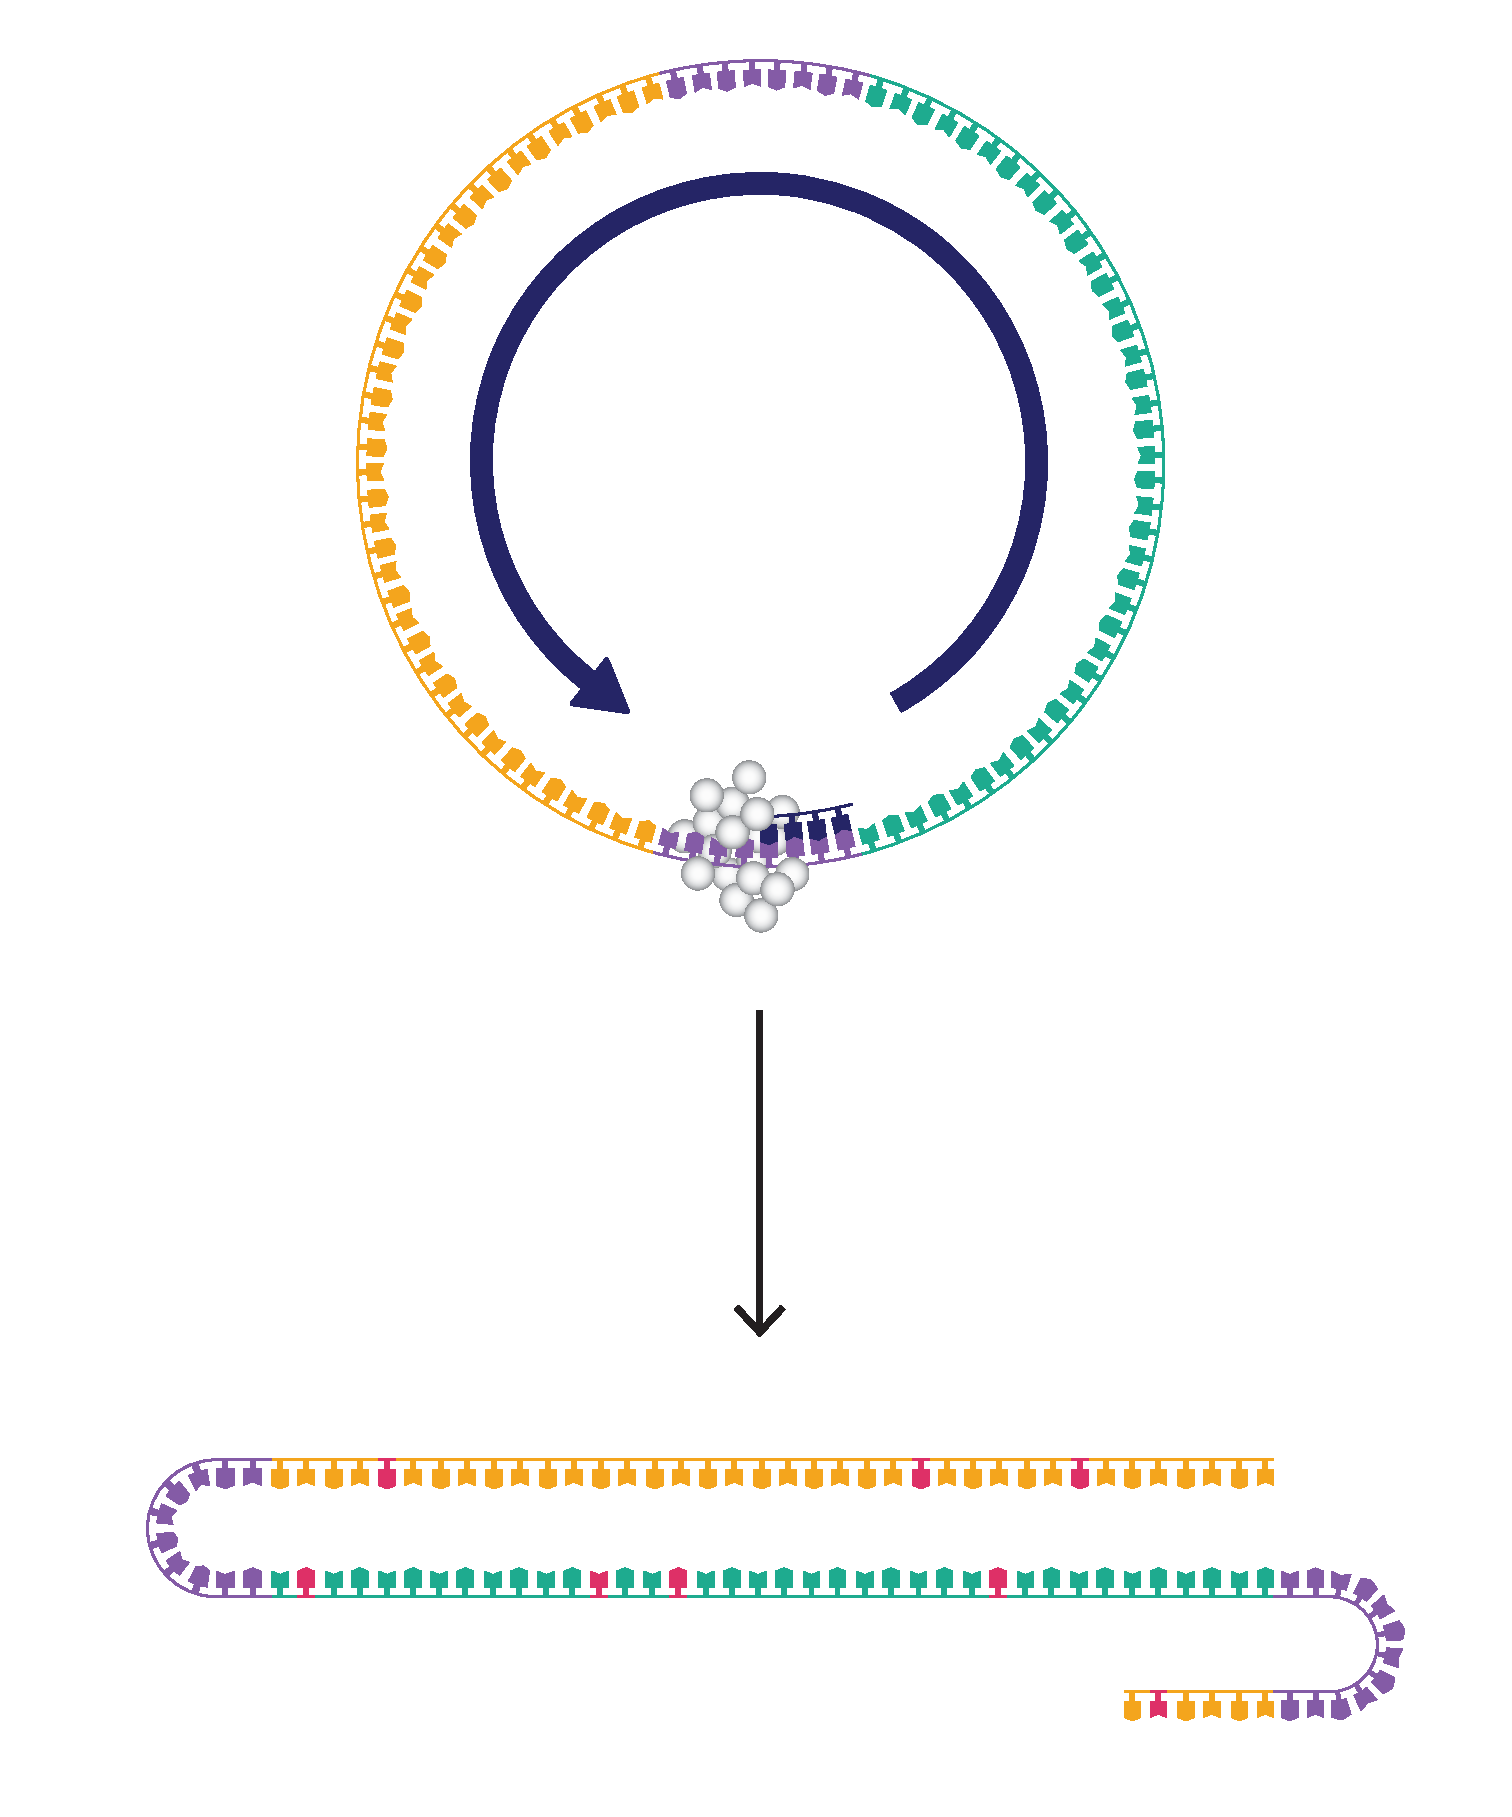
\includegraphics[width=0.8\textwidth]{Vector/CLR_sequencing.pdf}
\end{centering}
\floatfoot{DNAP used in CLR sequencing didn't have sufficient processivity to enable multiple-pass sequencing of read-of-insert greater than 10kb. Here, DNAP sequences the forward and reverse strand once.}
\end{figure}

At present, CCS sequencing with longer read length (>20kb) and higher read accuracy (Q20-Q30) \cite{Wenger2019-pw} is the method of choice. The major improvements in DNAP processivity and increase in the number of ZMWs per SMRTcell to 8 million and 25 million for the Sequel II and Revio sequencing instrument, respectively, enable high-throughput CCS sequencing. During the last fifteen years, from 2009 to 2024, the sequence throughput of SMRTcells has increased exponentially. The first generation of SMRTcells, with 150,000 ZMWs, produces approximately 112 million CLR bases. In contrast, the latest generation of SMRTcells with 25 million ZMWs generates around 250 billion CCS bases. These estimates were calculated assuming that half of the ZMWs are productive and produce CLR and CCS reads with an average read length of 1,500bp and 20kb, respectively. Consequently, the sequence throughput from the Revio sequencing instrument, using a single 25M SMRTcell, can achieve 30-fold CCS sequence coverage of a human genome for under one thousand dollars. Importantly, sequence throughput from a single 25M SMRTcell is not only sufficient to facilitate \textit{de novo} assembly \cite{Nurk2020-gu, Cheng2021-ij} but also enables haplotype phasing of \cite{Patterson2015-an} and detection of both germline mutations \cite{Poplin2018-ub} and base modifications \cite{Tse2021-or}.

\begin{figure}[htbp!]
\caption{CCS sequencing}
\label{figure:ccs-sequencing}
\begin{centering}
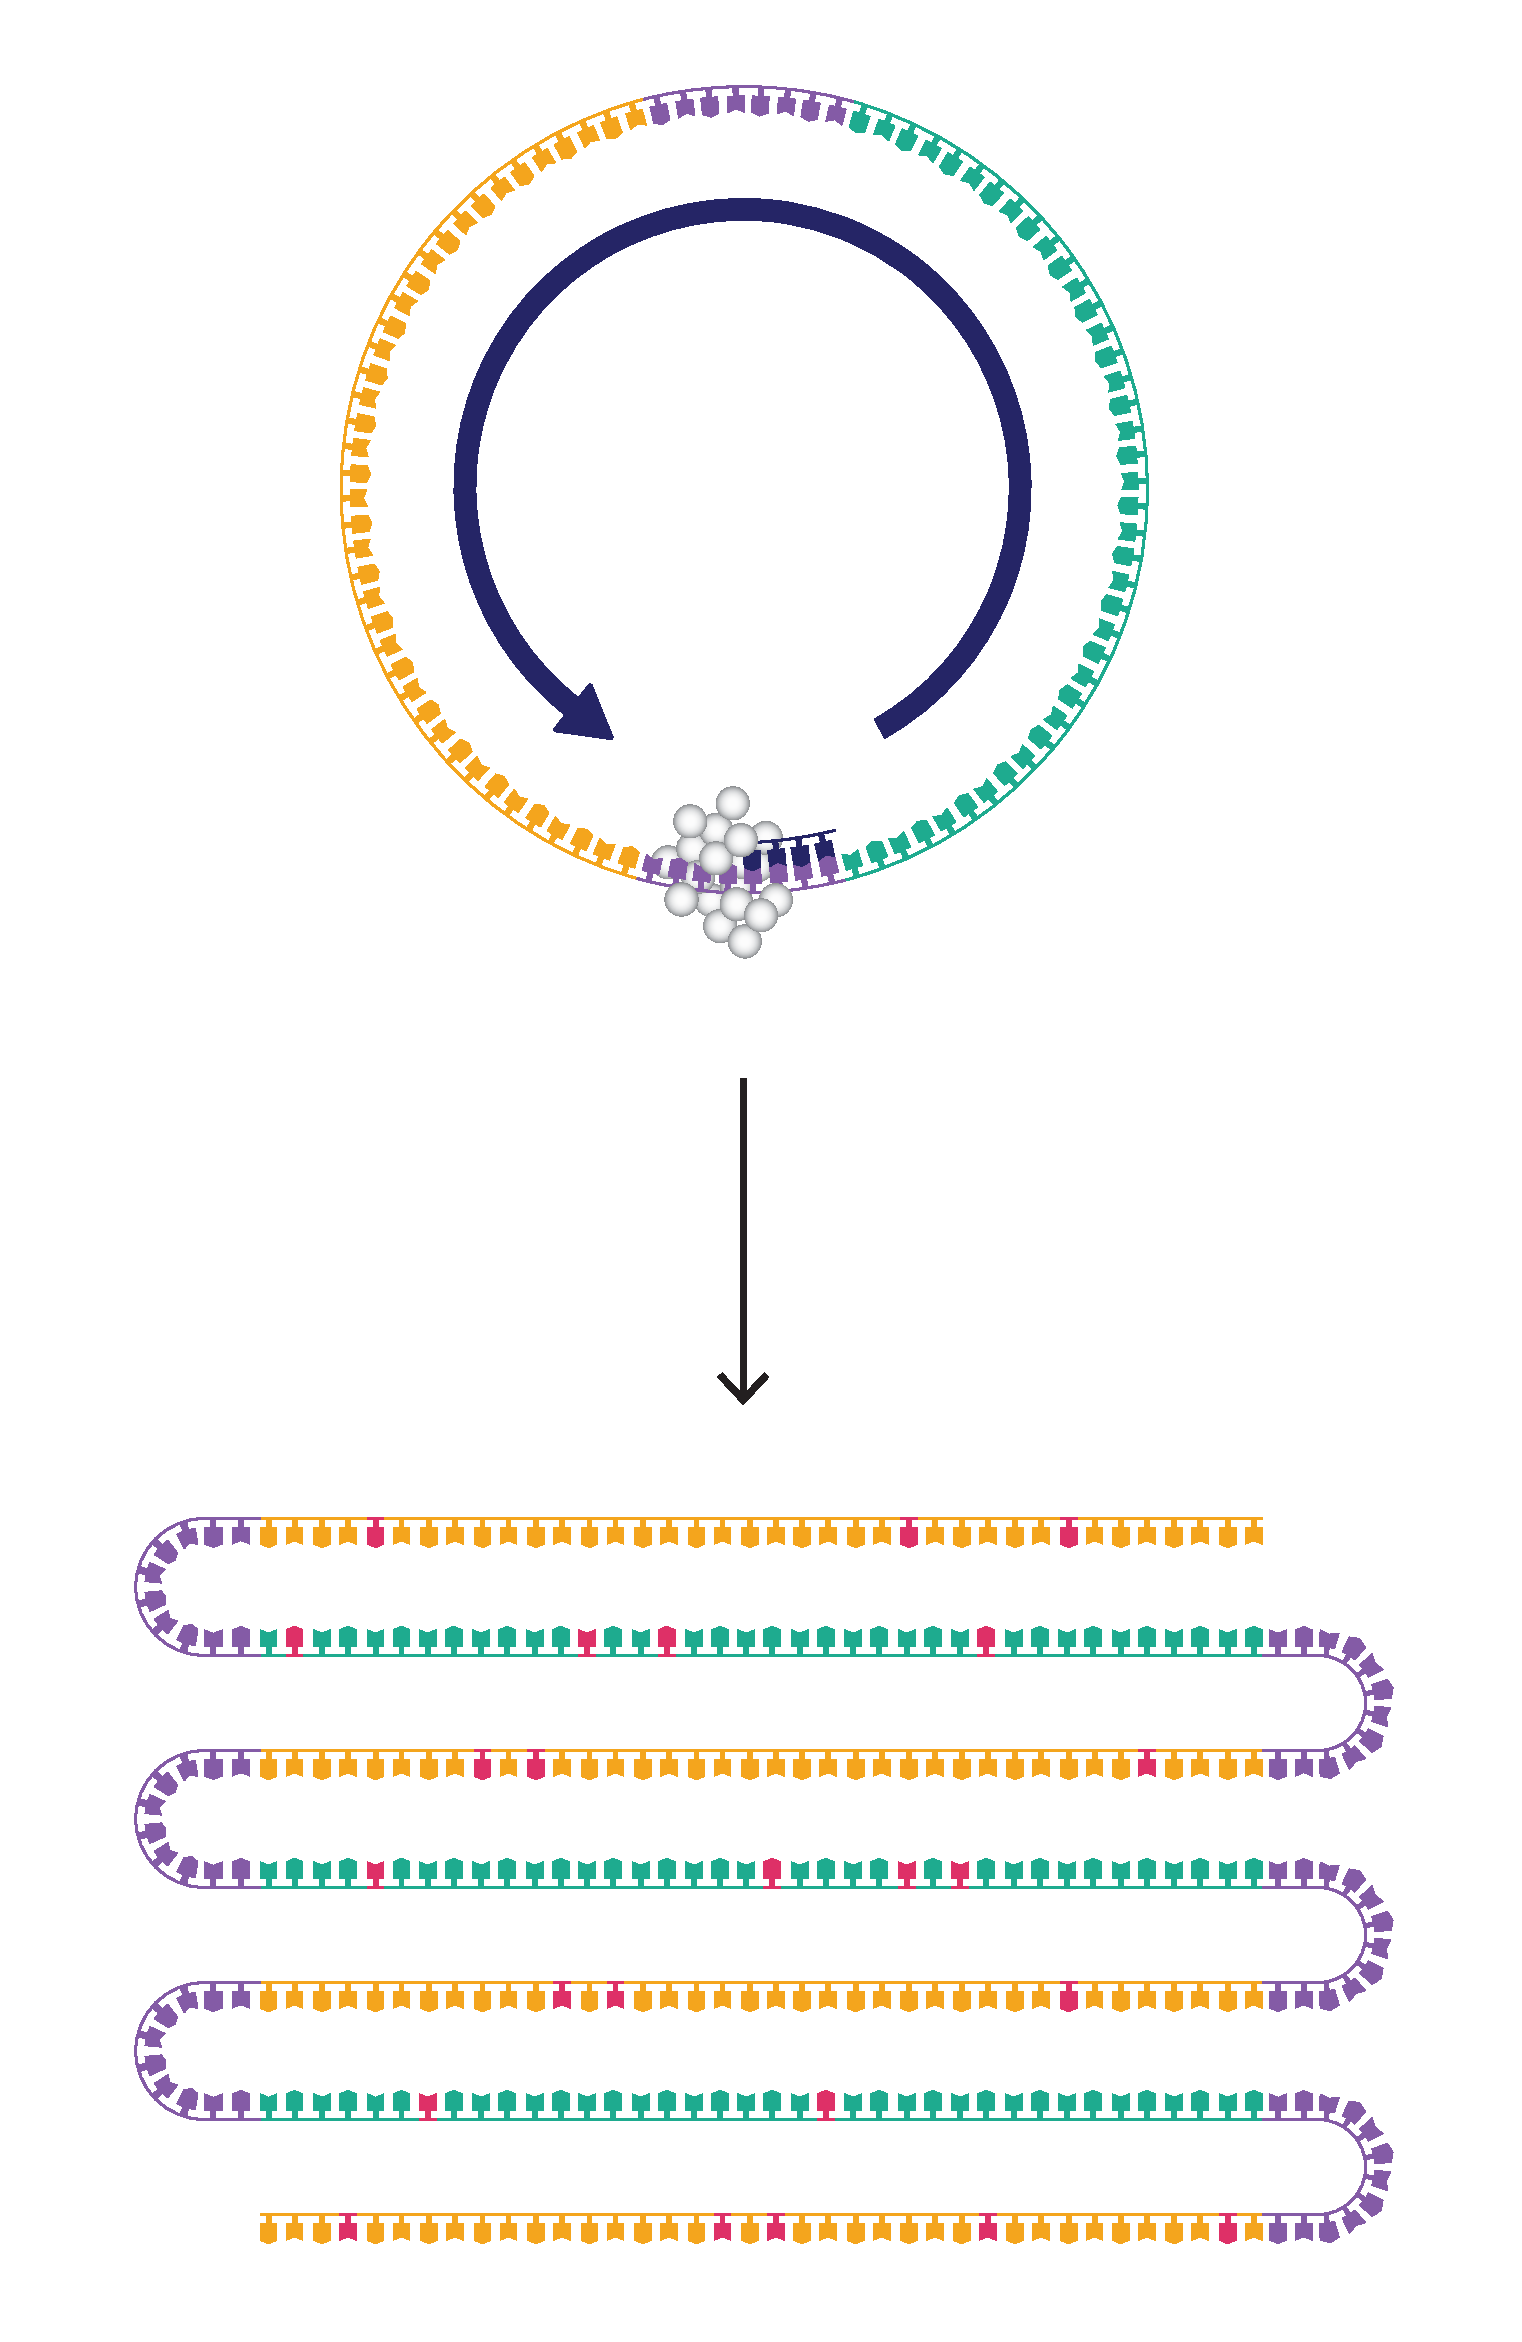
\includegraphics[width=0.8\textwidth]{Vector/CCS_sequencing.pdf}
\end{centering}
\floatfoot{In contrast, DNAP used in CCS sequencing have sufficient processivity to sequence a 20kb read-of-insert 10 to 16 times.}
\end{figure}

\subsection{Long-read sequencing applications}

The high error rate of CLR reads, coupled with lower sequence throughput compared to Illumina sequencing instruments, initially limited the applications of PacBio sequencing instruments to microbial genome assembly \cite{Chin2013-hp}, targeted BAC clone sequencing to close gaps in the human reference genome \cite{Huddleston2014-rs}, nucleotide-resolution structural variation detection \cite{}. The introduction of the P6-C4 chemistry and PacBio RSII instrument marked a significant milestone, leading to a substantial increase in CLR read length and sequence throughput \cite{Rhoads2015-pk}. This breakthrough enabled the successful assembly of larger and more repetitive mammalian genomes, including those of great apes such as gorillas \cite{Gordon2016-ho}, chimpanzees \cite{Kronenberg2018-wy}, and orangutans \cite{Kronenberg2018-wy}. Furthermore, CCS sequencing represents another significant advancement that enables us to explore previously unexplored biological phenomena.

\subsubsection{Genome assembly}

Genome assembly aims to determine the entire genetic information of an organism. It can be divided into four distinct stages: 1) shotgun or hierarchical shotgun sequencing and quality control, 2) all-to-all read alignments to find overlaps between reads and the generation of contigs from overlapping reads 3) the use of long-range information to order and orient contigs into scaffolds, and 4) finishing the genome through polishing and gap closing.

\textit{De novo} assembly algorithms perform all-against-all pairwise read alignments, identify overlaps between pairs of reads, generate an assembly graph from these overlaps, and then connect the reliable overlaps to produce contigs. The reliability of the overlap is dependent on the length of the overlap and the shared sequence identity between the overlap. The contiguity and completeness of contigs, resulting from these assembly algorithms, depend on the read length, sequence coverage and the length of overlap between reads, as modelled by the Lander-Waterman statistics \cite{Lander1988-hu}. Additionally, read length must be longer than the repeat length to ensure that unique sequences not found elsewhere in the genome flank the repetitive sequence in the read. If the read length is shorter than the repeat length, a repeat-induced false overlap is generated between reads that share a similar or identical repeat sequence. If these repeat-induced false overlaps are left unresolved, fragmented contigs are generated from the assembly graph. 

To minimise the number of potential assembly errors, the Human Genome Project (HGP) adopted hierarchical shotgun sequencing of 100-300 kb bacterial artificial chromosome (BAC) clones library to construct the human reference genome \cite{Lander2001-du}. In brief, genomic DNA is randomly fragmented into 100-300kb DNA fragments, followed by ligation into BAC vectors, which are then introduced into \textit{Escherichia coli} for DNA cloning. The resulting BAC library contains overlapping DNA fragments that can be sequenced, assembled, and connected to obtain the whole-genome sequence. To select overlapping BAC clones with minimal redundancies, also referred to as minimum tiling path of BAC clones, the position and orientation of BAC clones are determined through physical mapping techniques such as DNA fingerprinting \cite{} or fluorescent in-situ hybridization (FISH) \cite{}. Afterwards, BAC clones are Sanger sequenced, BAC contigs are assembled independent of each other and overlapping BAC contigs are ordered and oriented into a chromosome. In contrast to shotgun sequencing \cite{}, where reads derived from the entire genome are used to generate a set of contigs, hierarchical shotgun sequencing exclusively uses reads from the BAC clones to produce the BAC contig, thereby reducing the genome assembly problem to a local assembly challenge. Therefore, reference genomes produced through hierarchical shotgun sequencing approach boasts higher quality than that produced through shotgun sequencing approach. The HGP required international collaborations across multiple institutions to prepare, sequence and assemble the BAC clone library and hierarchical shotgun sequencing of BAC clones could not be easily replicated for other species. After the HGP, the first generation of assemblies were often generated using Illumina whole-genome sequencing and de Brujin graph assembly algorithms \cite{}. As expected, contigs generated from Illumina short reads were often fragmented as repeat-induced false overlaps could not be resolved. 

In contrast to Illumina short reads, CLR reads, with average read length greater than 10kb, from the PacBio RSII sequencing instrument could span the most commonly occurring repeats in the human genome such as $\sim$300 bp short interspersed nuclear element (SINE) and $\sim$5000 bp long interspersed nuclear element (LINE). Hence, CLR reads could be used to resolve repeat-induced false overlaps in the assembly graph to produce more complete and contiguous assemblies than that produced from short reads. A new generation of assembly algorithms based on de Brujin graph \cite{Lin2016-vl}, string graph \cite{Myers2005-ei, Chin2016-at} and overlap layout consensus (OLC) \cite{Koren2017-cq} were developed to leverage the availability of these long reads for \textit{de novo} assembly of microbial genomes\cite{Chin2013-hp, Bashir2012-cs} and large mammalian genomes \cite{Chin2016-at, Koren2017-cq}. In addition, long reads facilitate the identification of structural differences between the two haplotypes in a diploid genome and aid the unravelling of these divergences in the assembly graph. As a result, these new algorithms were able to produce haplotype phase contigs (haplotigs) and did not have to produce assemblies under the assumption that the sample has a haploid genome \cite{Chin2016-at}.  In short, the advent of CLR reads with read length greater than 10kb enabled the generation of more complete and contiguous assemblies than that produced from short reads, but the contigs were often fragmented where CLR reads could not resolve repeat-induced overlaps created from repeat sequences with sequence identity greater than 90\% such as segmental duplications, centromeric and telomeric repeats \cite{}. 

Recently, the introduction of CCS reads with higher base accuracy have completely fundamentally transformed how \textit{de novo} assemblies are performed. Compared to CLR reads, CCS reads are better at distinguishing more recently diverged repeats such as segmental duplications and hence, \textit{de novo} assemblies using CCS reads are often able to produce chromosome-arm level contigs \cite{}. In addition, the contiguity and completeness of these assemblies often exceeds that produced from hierarchical shotgun sequencing of BAC clones \cite{Nurk2020-gu, Cheng2021-ij}. 

The concurrent development of new sequencing and physical mapping technologies have enabled the routine generation of chromosome-length scaffolds \cite{}, and subsequently telomere-to-telomere assemblies \cite{}. For instance, optical genome mapping from BioNano Genomics uses a single restriction enzyme or multiple restriction enzymes to introduce nicks to a linearized high molecular weight DNA. Afterwards, nucleotides labelled with fluorescent dyes are incorporated to these restriction enzyme sites, and fluorescent microscopy is used to image these single molecules of DNA to produce physical maps. Similar to how overlapping reads in an assembly graph can be used to produce a contig, overlapping physical maps can be used to generate a genome map, which can be used to order and orient contigs into chromosome-length scaffolds \cite{}. The fragmentation rate of genome maps increases with the number of restriction enzyme sites on the complementary strand \cite{}, while contigs are fragmented when read length is insufficient to resolve repeat-induced false overlaps in the assembly graph. The independent mechanism of fragmentation makes genome maps and contigs highly complementary and enables one of the two methods to span regions of the genome where one method cannot. 

Lately, high-throughput chromatin conformation capture (Hi-C) sequencing has replaced physical mapping as a more cost-effective method to organize contigs into scaffolds. Chromosome conformation capture (3C) method, and later Hi-C sequencing, was originally developed to study the local and global three-dimensional conformation of the genome, respectively \cite{}. The method relies on crosslinking chromatin through formaldehyde fixation to prevent additional changes to the genome architecture. The cells with crosslinked chromatins are then lysed and DNA is fragmented using a restriction enzyme. Afterward, ligation between cross-linked DNA fragments is promoted, resulting in ligation products that contain chimeric molecules consisting of DNA segments that are adjacent to each other in three-dimensional space, but distant in one-dimensional space. Hi-C libraries are produced from these ligation products and the resulting paired-end reads are processed to measure the contact frequencies between distant segments of genome \cite{}. Hi-C sequencing can be conceptualized as mate pair sequencing \cite{}, with a distribution of insert sizes and with the upper limit defined by the length of the chromosome. 

Research into the genomic architecture using Hi-C sequencing has revealed how the genome is organised \cite{}, how the organisation changes to regulate gene expression \cite{}, and how a number of different proteins orchestrate the changes in the conformation of the genome \cite{}. Hi-C scaffolding algorithms leverage several key properties of genome organisation to not only correct contig mis-assemblies but also to arrange contigs into scaffolds. These key characteristics include higher intra-chromosome contact frequency compared to inter-chromosome contact frequency, and a decrease in contact frequency between DNA segments with increasing distance in one-dimensional space. The former allows contigs from the same chromosome to be grouped together, while the latter enables the sorting of contigs from the same chromosome \cite{}. In addition, aberrant contact frequencies between DNA segments can be used to identify contigs with mis-ordered or mis-joined sequences \cite{}. If un-resolved mis-assemblies exist or if contigs are not adjoined where possible, manual inspection of the Hi-C contact matrix can also correct the remaining issues \cite{}. The ability to identify and correct mis-assemblies before scaffolding, group and organise contigs into scaffolds, and to visually evaluate the quality of scaffolds has improved the contiguity of assemblies and expedited the production of chromosome-length scaffolds. 

Together, CCS and Hi-C sequencing have dramatically improved not only the completeness, but also the contiguity of reference genomes. However, these reference genomes remain incomplete with missing sequence, also known as gaps, and imperfect with mis-assemblies such as false sequence collapse or expansion. Fortunately, the development of ultra-long read (>100kb) library preparation and nanopore sequencing has allowed us to close remaining gaps in the reference genome \cite{}. Full-length sequencing and successful \textit{de novo} assembly of BAC clone inserts that tile the chromosome Y centromere, which has been recalcitrant to assembly since the human genome project, highlights one of the many successful use cases of ultra-long nanopore reads \cite{}. Additionally, ultra-long read sequencing has been critical in the completing the gapless T2T-CHM13 genome, which includes the short arms of five acrocentric chromosomes and centromeric satellite array, adding nearly 200 million new bases to the human genome \cite{}.

The assembly of a gapless and complete haplotype-resolved genome represents one of remaining challenges in genomics research, and new sequencing methods and algorithms have started to address this problem. For instance, assembly algorithms are able to use CCS reads not only to distinguish recently diverged repeats such as segmental duplications, but also distinguish sequences originating from different haplotypes \cite{}. In addition, if Hi-C reads are provided to the assembly algorithm, assembly graph can be phased and contigs from the same parental chromosome can be grouped and returned together as haplotigs \cite{}. Finally, if both maternal and paternal genomes are sequenced, maternal- and paternal-specific kmers can be identified and be used to bin CCS reads prior to assembly to produce haplotigs \cite{}. 

\subsubsection{Germline and somatic mutation detection}

To date, several studies have used both CLR and CCS Reads to analyse germline SNPs, insertions and deletions (indels) and structural variations with event sizes greater than 50bp. For instance, CHM1 CLR reads were used to identify approximately 26,000 structural variations that were recalcitrant to detection using short reads \cite{Chaisson2015-zz}. The number of structural variations detected with long reads is at least double that detected with short reads. Moreover, even though the number of structural variations is orders of magnitude smaller than the number of SNPs and indels, they can alter a greater number of bases and have a more pronounced impact on an individual's phenotype \cite{Weischenfeldt2013-tl}. Additionally, structural variations can induce conformational changes in the three-dimensional configuration of the genome, promote contact between gene promoters and enhancers, and thereby alter gene expressions \cite{Spielmann2018-fm}.

The diagnosis rate of rare genetic diseases is estimated to be approximately 30-40\% with short read sequencing \cite{Wright2023-et}, and new germline mutation detection and interpretation methods have only marginally improved the diagnosis rate, suggesting that perhaps a completely new sequencing method is required to dramatically improve the diagnosis rate. There is no question that structural variation detection with long reads offers better sensitivity and specificity compared to short reads. Longer read length enables unambiguous read alignment to the reference genome and allows access to previously inaccessible regions of the genome. Since a head-to-head comparison between short- and long-read sequencing for diagnosis rare genetic diseases has not been conducted, the diagnosis rate of rare genetic disease with long reads remains unknown. However, a couple of studies demonstrate the potential of SMRT sequencing to not only identify the sequences responsible for the Mendelian disease, but also elucidate the underlying mechanism. For instance, repeat expansions and accompanied hypermethylation are common causes of neurological diseases \cite{Zhou2022-ci}. Analysis of short tandem repeat (STR) expansions using long read sequencing in individuals diagnosed with spinocerebellar ataxia type 10 (SCA10) has revealed that both the repeat sequence composition and the number of repeat expansions influence disease severity \cite{McFarland2015-qh}. Unsurprisingly, the ability to haplotype phase and detect both germline mutations and base modifications using SMRT sequencing is renewing interest to apply SMRT sequencing for identification of pathogenic mutations in individuals diagnosed with rare genetic diseases \cite{Miller2021-lt}. 

Although long-read sequencing technologies offer numerous advantages compared to short-read sequencing technologies for somatic structural rearrangement detection, long reads have been under-utilised in somatic mutation detection. To date, only a handful of samples have been sequenced to interrogate somatic structural rearrangements using long reads \cite{Nattestad2018-tr, Sakamoto2020-nq, Fujimoto2021-kc}. Moreover, somatic substitution and indel detection algorithms, to our knowledge, have not been developed to leverage CLR or CCS reads. Hence, I believe that a series of method development is required to enable the adoption of long-read sequencing for cancer genomics research.

\section{Tree of Life}

The Tree of Life is a recurring cultural and religious symbol in human history, and Charles Darwin first used the Tree of Life to illustrate the interconnectedness of different species through a shared common ancestor, and the emergence and extinction of new species through natural and sexual selection (Figure \ref{figure:tree-of-life}) \cite{Darwin1859}. 

Since the publication of \textit{On the Origin of Species} \cite{Darwin1859}, one of Darwin's seminal works, a number of scientific milestones have established that all living species on Earth are derived from a common ancestor. Firstly, nucleic acid has been unequivocally determined to be the universal carrier of genetic information \cite{Avery1944-lr}. Secondly, the same genetic code, where a triplet of nucleotides encode one of the twenty amino acids, is universally employed across all forms of life \cite{Woese1968-lr}. Thirdly and finally, all forms of life use a similar set of machineries to perform transcription and translation, the production of messenger RNA (mRNA) and protein from mRNA, respectively \cite{}

The process of natural selection relies on intra-species competition, where individuals with diverse genotypes and phenotypes vie for survival. Those better adapted to the environment survive, reproduce offspring, and thereby propagate the mutations advantageous for survival. Ongoing germline mutational processes introduce new mutations, the source of raw material, for natural selection. Unfortunately, the prohibitive cost of clone-by-clone sequencing and the inability to produce high-quality reference genome using short-read sequencing have prevented the study of germline mutational processes across the Tree of Life. Additionally, the challenges of somatic mutation detection in normal tissues have limited the examination of somatic mutational processes. 

\subsection{Peto’s paradox}

The study of somatic mutations and mutational processes in other species is a fascinating area of research that sheds light on the underlying mechanisms of aging and the occurrence of cancer. Sir Richard Peto observed that there is no clear correlation between the number of cells and the incidence of cancer in other animals \cite{Peto2016-wf, Vincze2022-tw}. Because somatic mutational processes alter the genome of individual cells, and the number of somatic mutations increases with age, it might be expected that larger animals with a greater number of cells and long-lived species would have an elevated risk of developing cancer. However, elephants provide an interesting counter example. Elephants have over one hundred times the number of cells compared to humans, but they have a cancer mortality rate of 4.81\%, in contrast to the 11-25\% cancer mortality rate in humans \cite{Abegglen2015-ao}. The comparison of the elephant and human genome has revealed the potential genomic differences that might explain the discrepancies in cancer mortality rate. In contrast to the human genome, which carries 2 copies of the TP53 gene, the elephant genome boasts 20 copies \cite{Sulak2016-ld}. Because the TP53 gene, a critical tumour suppressor gene for maintaining genome stability \cite{Vousden2009-wd}, is frequently mutated in tumours to either silence gene expression or abrogate gene function \cite{}, the higher number of TP53 genes in the elephant genome is believed to be one of the primary reasons why elephants have a lower incidence of cancer. Peto’s paradox remains unresolved and unravelling the underlying mechanism would require comparative genomic analysis between high-quality reference genomes to identify the unique and common solutions developed in each species to prevent tumourigenesis. 

\subsection{Somatic mutation theory of ageing}

The somatic mutation theory of ageing suggests that the gradual accumulation of somatic mutations leads to a decline in cellular function, ultimately contributing to the ageing process \cite{Szilard1959-ru}. This theory also implies that shorter-lived species will have a higher somatic mutation rate than longer-lived species. A recent study of somatic mutation rate in colonic crypt across various mammalian species of different ages and lifespans has determined that the somatic mutation rate is inversely proportional to the lifespan of mammalian species \cite{Cagan2022-yn}, confirming that longer-lived species have a lower somatic mutation rate than short-lived species. The extent to which this relationship between species’ lifespan and somatic mutation rate holds true remains uncertain, particularly concerning whether the relationship is universal across mammalian species or extends to species from other taxonomic classifications. The study of somatic mutational processes and somatic mutation rate across the Tree of Life would be required to answer this question. 

\subsection{Darwin Tree of Life project}

As discussed above, the ability to produce chromosome-length scaffolds, using the latest sequencing technologies and assembly algorithms, has brought new enthusiasm to assemble high-quality reference genomes for all vertebrates \cite{Rhie2021-dq} and all eukaryotic diversity on Earth \cite{Lewin2018-zf}. Recently, the Wellcome Sanger Institute announced the Darwin Tree of Life (DToL) project to build reference genomes for all 70, 000 eukaryotic species in Britain and Ireland using a combination of sequencing and physical mapping technologies \cite{Darwin_Tree_of_Life_Project_Consortium2022-ma}. To date, the DToL project has publicly released data and reference genomes for approximately 1600 eukaryotic species. The availability of high-quality reference genomes through the DToL project presents a new opportunity to study germline and somatic mutational processes across the Tree of Life and address questions that could not be answered, not because of the lack of imagination, but because of prohibitive cost of high-quality reference genome production through hierarchical shotgun sequencing. 

\section{Thesis objectives}

This PhD thesis is a product of the unique opportunity presented by the DToL project, and the remainder of the thesis is organised as follows. In chapter 2 \section{}, I assess the potential for single-molecule somatic mutation using CCS reads, where a single observation of the alternative allele is sufficient to call it as a somatic mutation, rather than an error. I also introduce himut, a method that leverages CCS read length and base accuracy to detect somatic mutations, agnostic of clonality and species. In chapter 3 \section{},  I use himut and deepvariant to call germline and somatic mutations from various eukaryotic species, leveraging CCS reads and high-quality reference genomes publicly available through the DToL project. I also describe newly discovered germline and somatic mutational signatures, and detail mutational signatures that are conserved across different taxonomic classifications.

